% !TEX root = main.tex

\section{语义图像分割}
以前的CNN都是对整幅图像进行分类,但现在则希望对\emph{单一像素}进行分类,实现图片中各个物体的分离,这在自动驾驶、智能家居和医学图像方面都有广泛用途。

传统采用滑动窗口(sliding window)的方法,取每个像素周围一小块,送入CNN中进行分类,此即利用周围特征进行分类。
但是这种方法非常的低效,有大量重复的区域进行计算,同时只能捕获一些局部特征。

\subsection{全卷积}
尝试将输出变为$C$个通道,每个通道对应一个目标类别。
但如果全部层都直接使用卷积操作,那么\textbf{计算量和内存消耗}将很大,同时也难以捕获\textbf{更大的感受野}。

因此采用缩放技术,即\newterm{降采样}(downsampling)和\newterm{上采样}(upsampling)构成编码-解码(encoder-decoder)框架,从而更容易捕获不同层次的特征。
\begin{figure}[H]
\centering
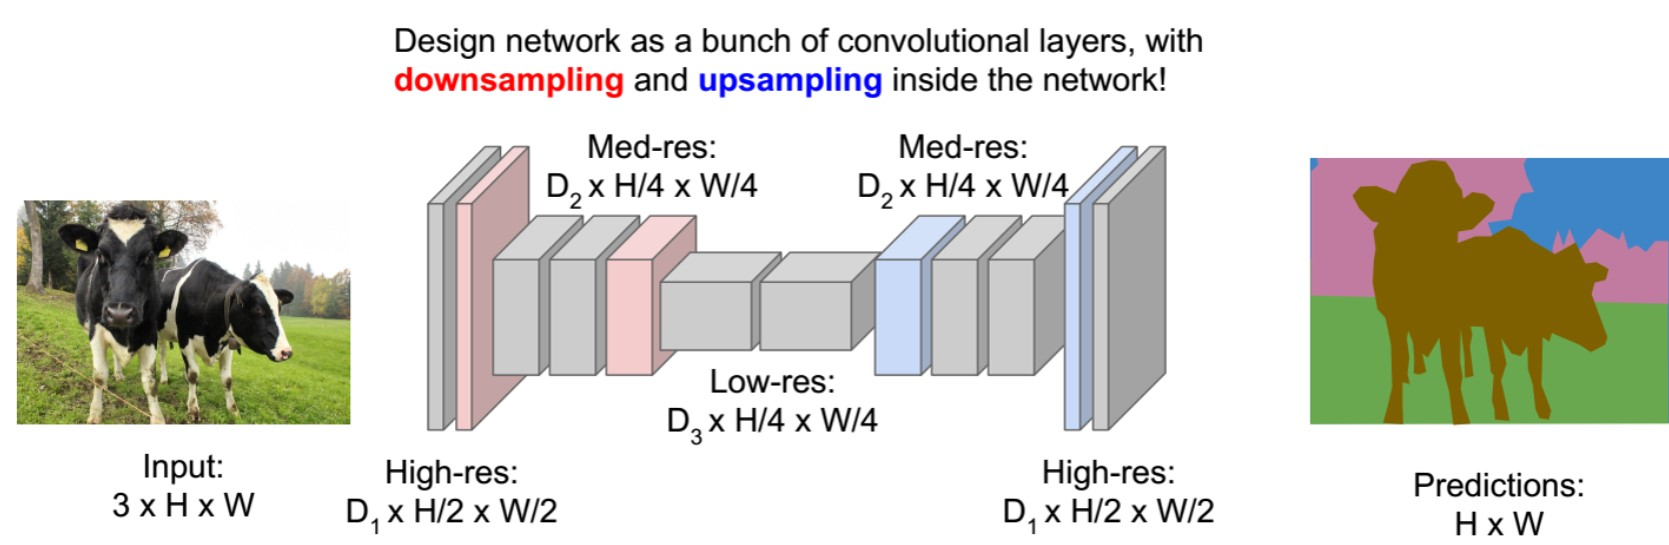
\includegraphics[width=0.9\linewidth]{fig/encoder-decoder.jpg}
\caption{编码-解码框架}
\end{figure}

通过类似池化的操作可以实现降采样,而上采样则通过\newterm{反卷积}(transposed convolution / deconvolution)实现。
如下图,改变步长和填充(padding)即可以实现反向卷积。
\begin{figure}[H]
\centering
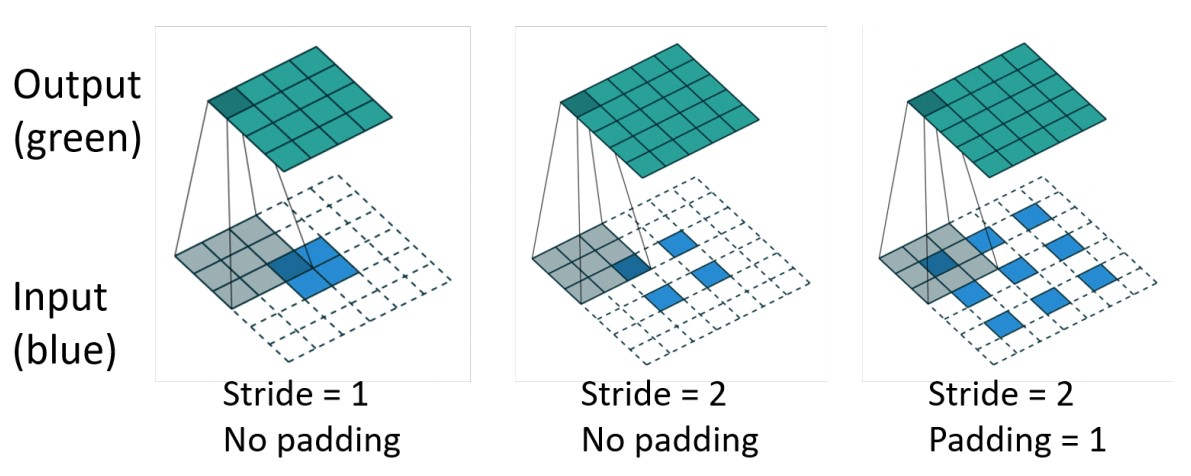
\includegraphics[width=0.8\linewidth]{fig/deconvolution.jpg}
\caption{反卷积}
\end{figure}

\subsubsection{FCN}
进而得到了全卷积网络(FCN)\cite{long:fcn},直接学习\textbf{像素到像素的映射},同时也避免CNN对输入尺寸的限制。
% https://zhuanlan.zhihu.com/p/32037333
\begin{figure}[H]
\centering
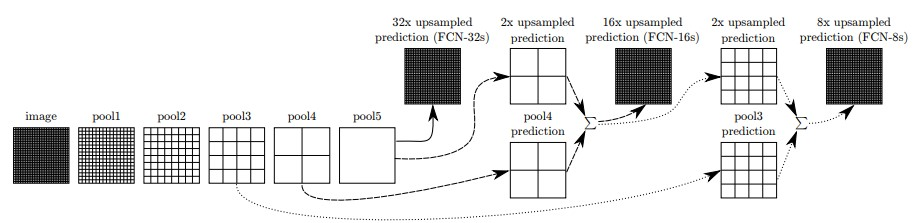
\includegraphics[width=\linewidth]{fig/fcn.jpg}
\end{figure}

这里最简单的FCN-32就是将传统CNN最后面的全连接层全部替换为卷积层,但由于通过降采样已经是分辨率很低的特征,因此通过反卷积出来的效果也不会太好。
FCN-16和FCN-8则是将\textbf{低分辨率特征和高分辨率的特征进行整合},进而输出更加细致的分割图像。

\subsubsection{U-Net}
但FCN得到的结果依然不够精细,对图像中细节不敏感。

而U-Net\cite{olaf:unet}则是通过\textbf{相同次数的下/上采样},\textbf{编码块和解码块的跳层连接}实现更优的语义分割。
\begin{figure}[H]
\centering
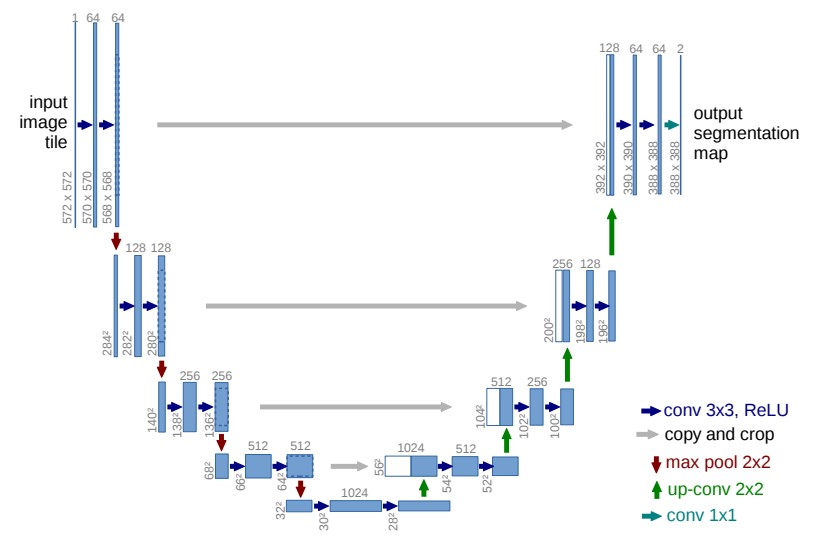
\includegraphics[width=0.8\linewidth]{fig/unet.jpg}
\end{figure}

通过U-Net和Dense ResNet结合可以实现更加高的性能,即Tiramisu Net\cite{simon:tiramisu_net_2016}。

\subsubsection{PSPNet}
但FCN不能很好地考虑全局信息,导致分割失误。
而PSPNet\cite{zhao:pspnet_2017}则分为以下三步:
\begin{itemize}
	\item 编码器:采用\newterm{扩张/空洞卷积}(dilated/atrous),可以有更大的感受野
	\begin{figure}[H]
	\centering
	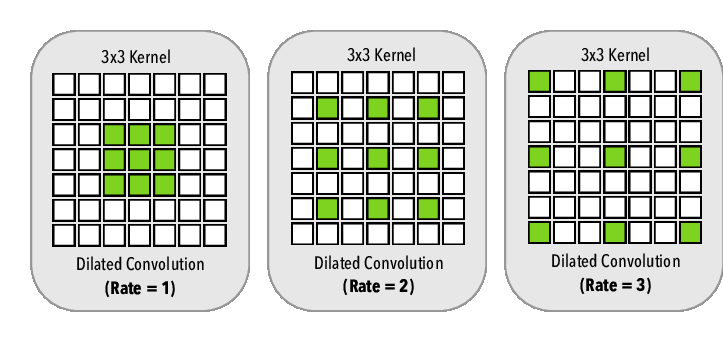
\includegraphics[width=0.6\linewidth]{fig/dilated_convolution.png}
	\end{figure}
	\item 金字塔池化:在\textbf{不同尺度}进行池化操作
	\item 合并:将上采样结果和原始编码器结果进行合并,这个操作继承了之前的网络的优点(跳连),同样实现捕获\textbf{不同分辨率}的特征
\end{itemize}

\begin{figure}[H]
\centering
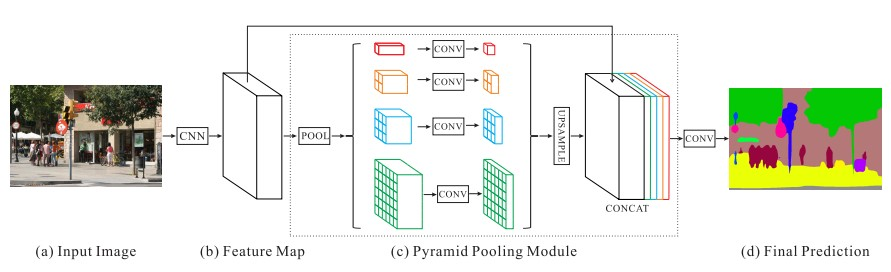
\includegraphics[width=0.9\linewidth]{fig/pspnet.jpg}
\end{figure}

\subsection{空洞卷积}
除了利用编码-解码架构,还可直接采用空洞卷积,\textbf{避免编解码的损耗},此即DeepLab\cite{chen:deeplab_2016}的思想。
% DeepLab 语义分割模型 v1、v2、v3、v3+ 概要(附 Pytorch 实现) - Uno Whoiam的文章 - 知乎
% https://zhuanlan.zhihu.com/p/68531147
\begin{itemize}
	\item 前面的特征提取部分同VGG16,然后改成用空洞卷积提取特征,维持较高的分辨率
	\item 采用\textbf{双线性插值}实现上采样,恢复原图大小
	\item 用条件随机场(CRF)使得分类结果边缘更加精细
\end{itemize}
\begin{figure}[H]
\centering
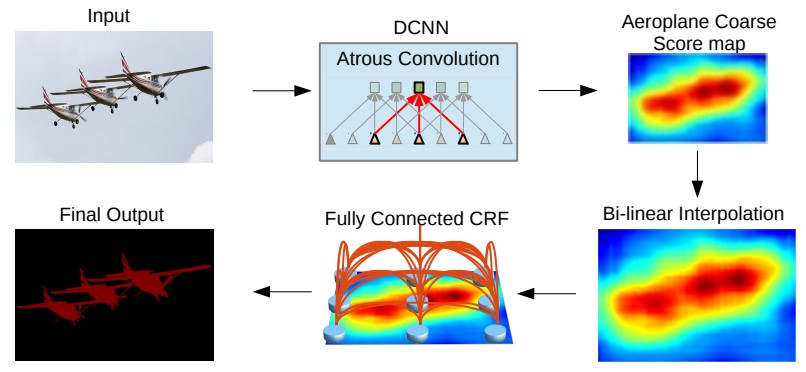
\includegraphics[width=0.7\linewidth]{fig/deeplabv1.jpg}
\end{figure}

v2版本的DeepLab则在模型最后添加了空间\textbf{金字塔}型的空洞卷积(ASPP),类似PSPNet,用于捕获\textbf{不同尺度}的特征。
\begin{figure}[H]
\centering
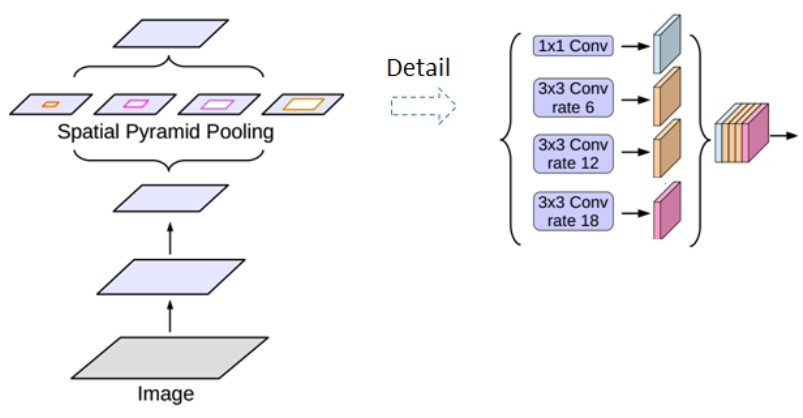
\includegraphics[width=0.6\linewidth]{fig/deeplabv2.jpg}
\end{figure}

v3则改动了以下几点:
\begin{itemize}
	\item Multi-grid策略:在模型最后添加几层不同rate的空洞卷积
	\item 将批归一化添加到ASPP
	\item 全局池化层+conv$1\times 1$
\end{itemize}
\begin{figure}[H]
\centering
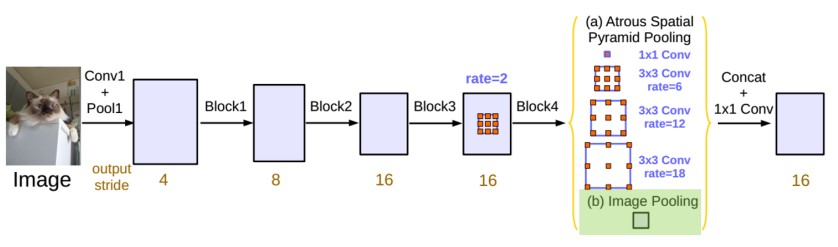
\includegraphics[width=0.8\linewidth]{fig/deeplabv3.jpg}
\end{figure}

再到v3+\cite{chen:deeplabv3p_2018},则是将空洞卷积和编码-解码架构进行结合。
编码器最后使用ASPP,解码器采用双线性插值上采样,同时前后\textbf{跳连}从而获得更加精细的结果。
\begin{figure}[H]
\centering
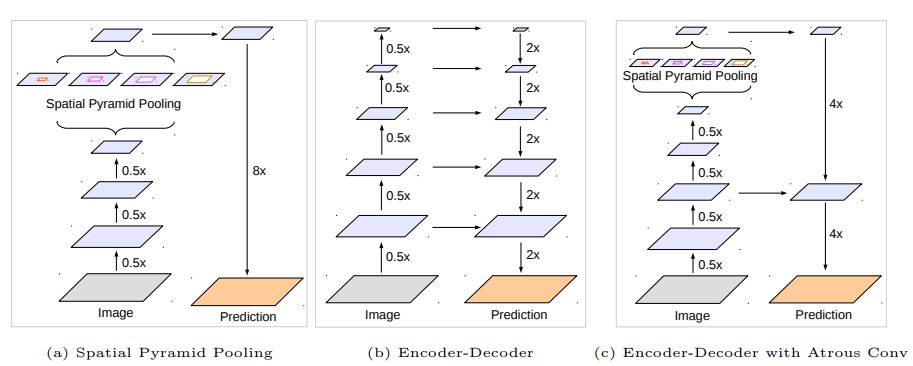
\includegraphics[width=\linewidth]{fig/deeplabv3+.jpg}
\end{figure}